\clearpage
\subsection*{PPL de Minimizare – dietă}
\paragraph{}
Un student poate găti doar cartofi, piept de gaină, hriscă și ouă. Să se elaboreze o dietă cât mai echilibrată astfel încât studentul să stupravețuiasca pană în semestrul următor. Datele problemei sunt în tabelul de mai jos.


\paragraph{}
\begin{figure}[h]
\begin{center}
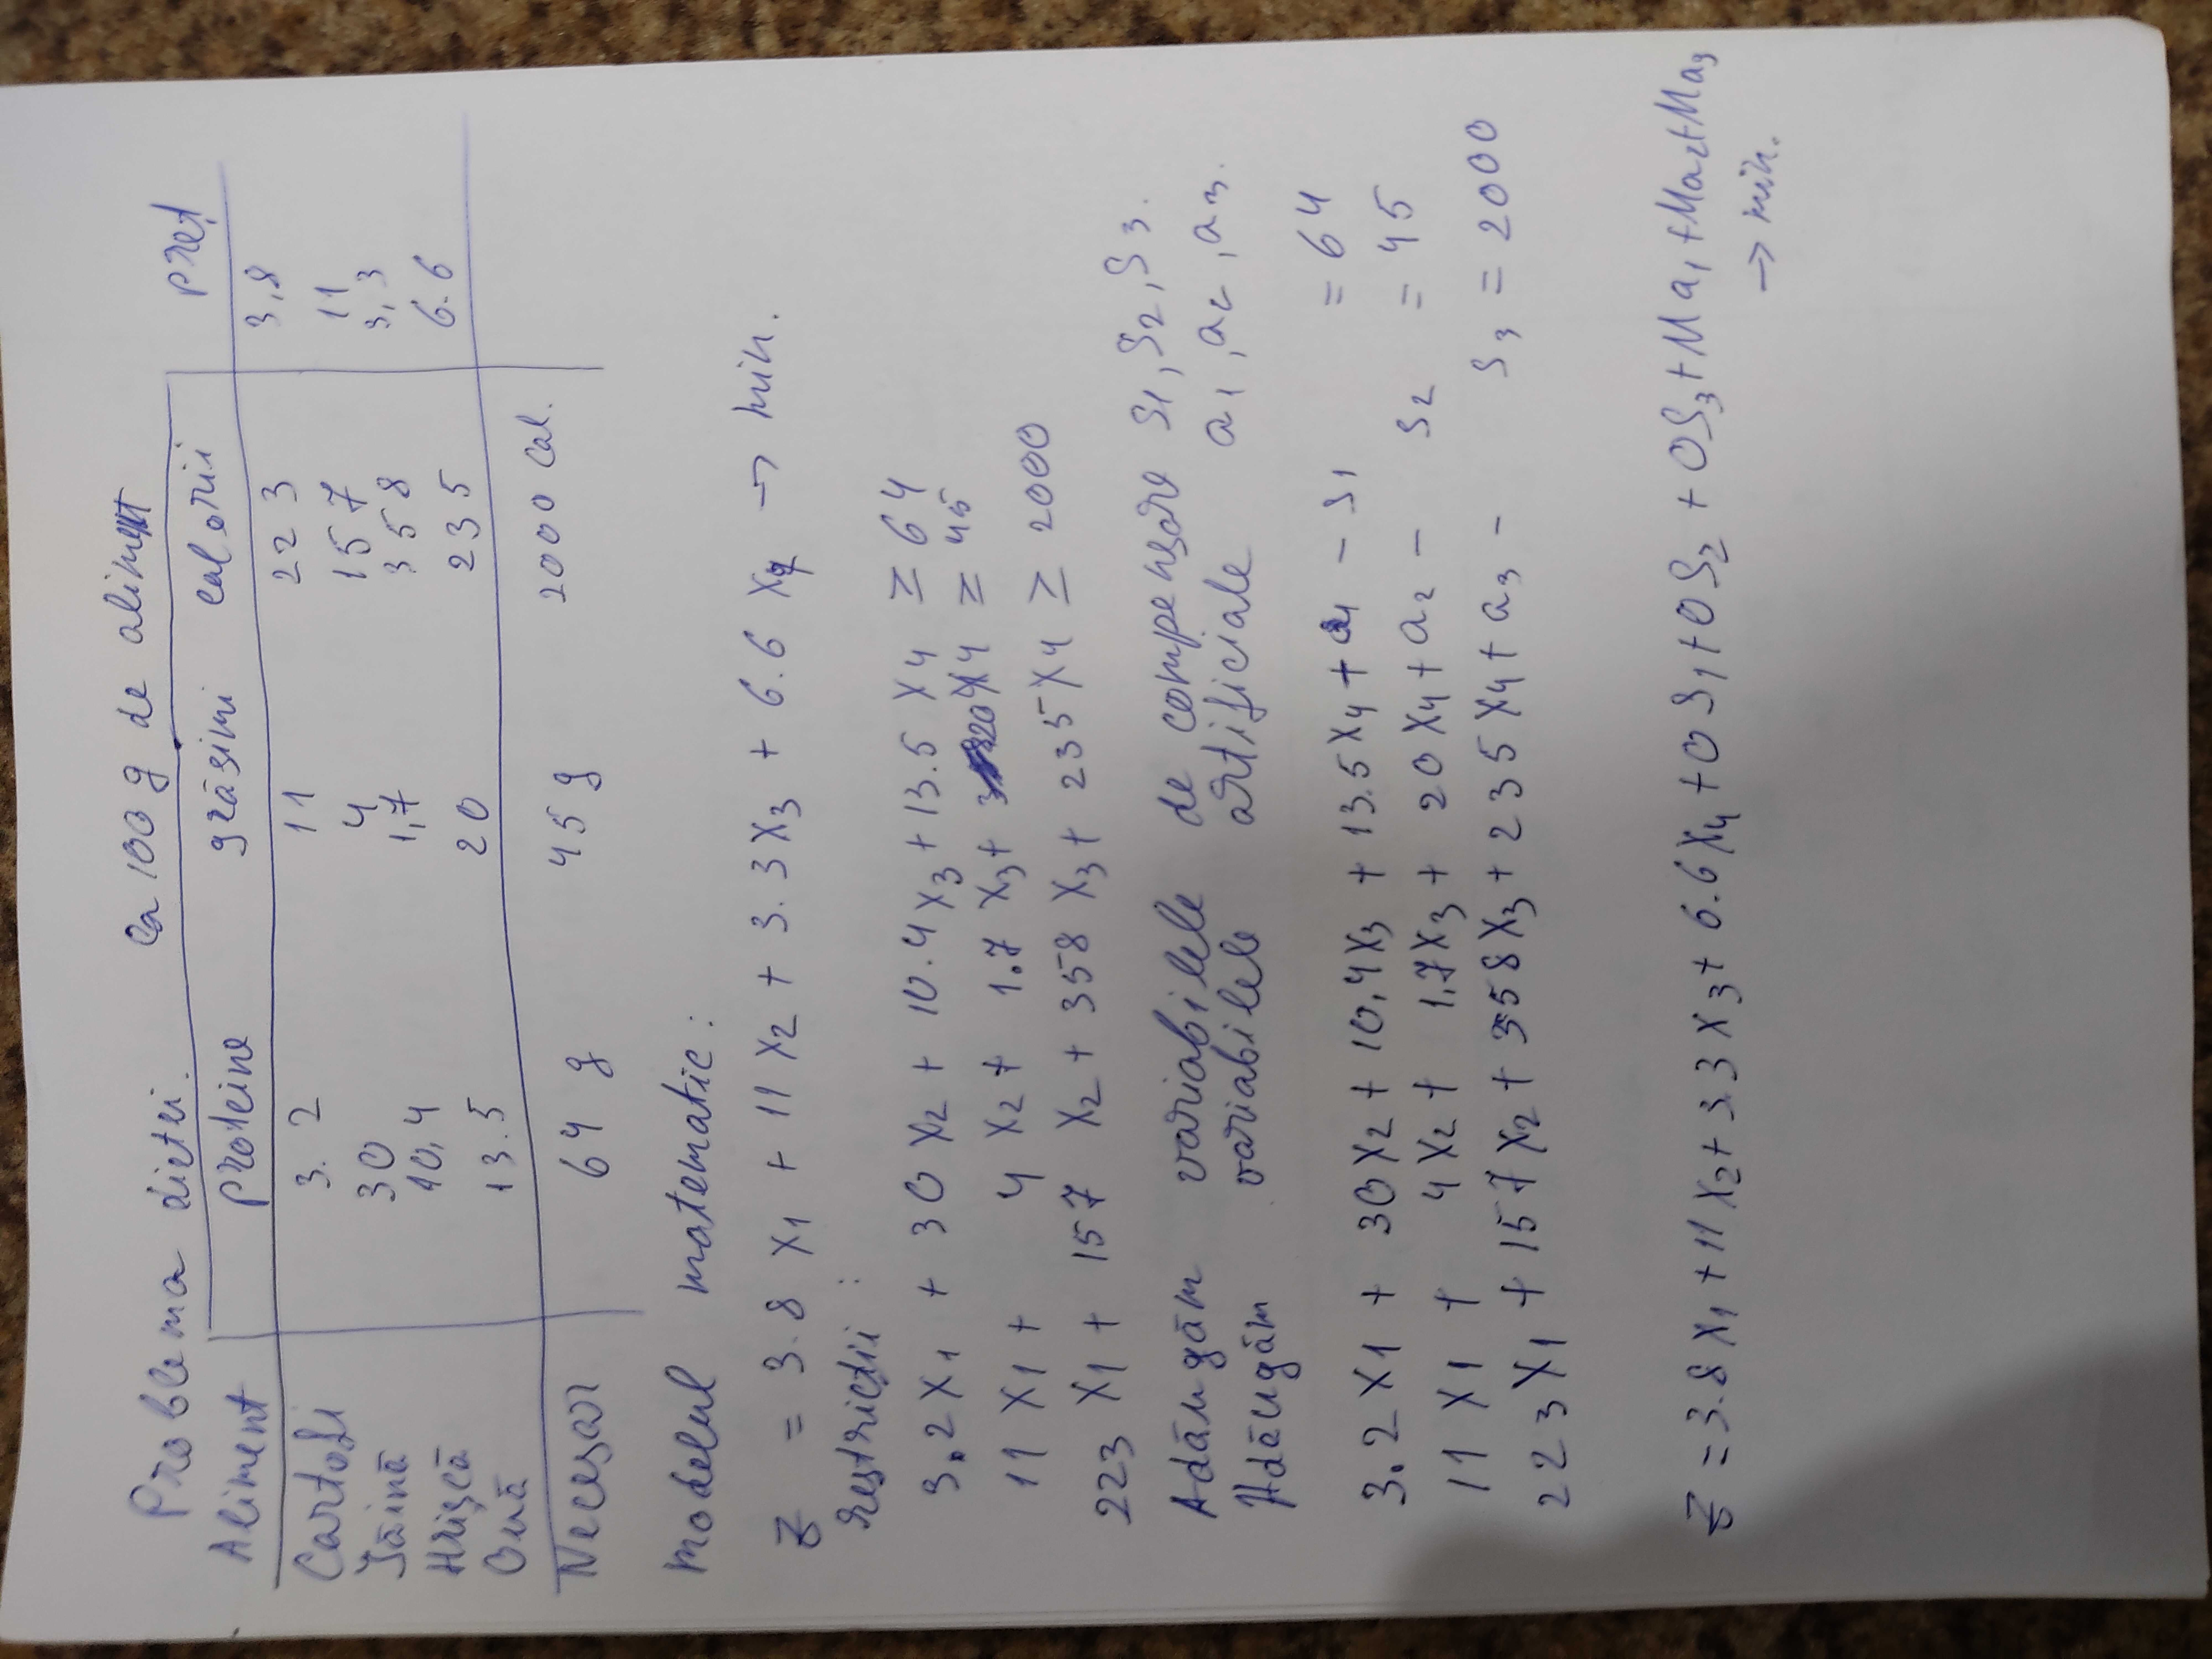
\includegraphics[width=22cm, angle =-90]{3}
\caption{Datele problemei și modelul matematic} 
\label{fig:3}
\end{center}
\end{figure}

\paragraph{}
\begin{figure}[h]
\begin{center}
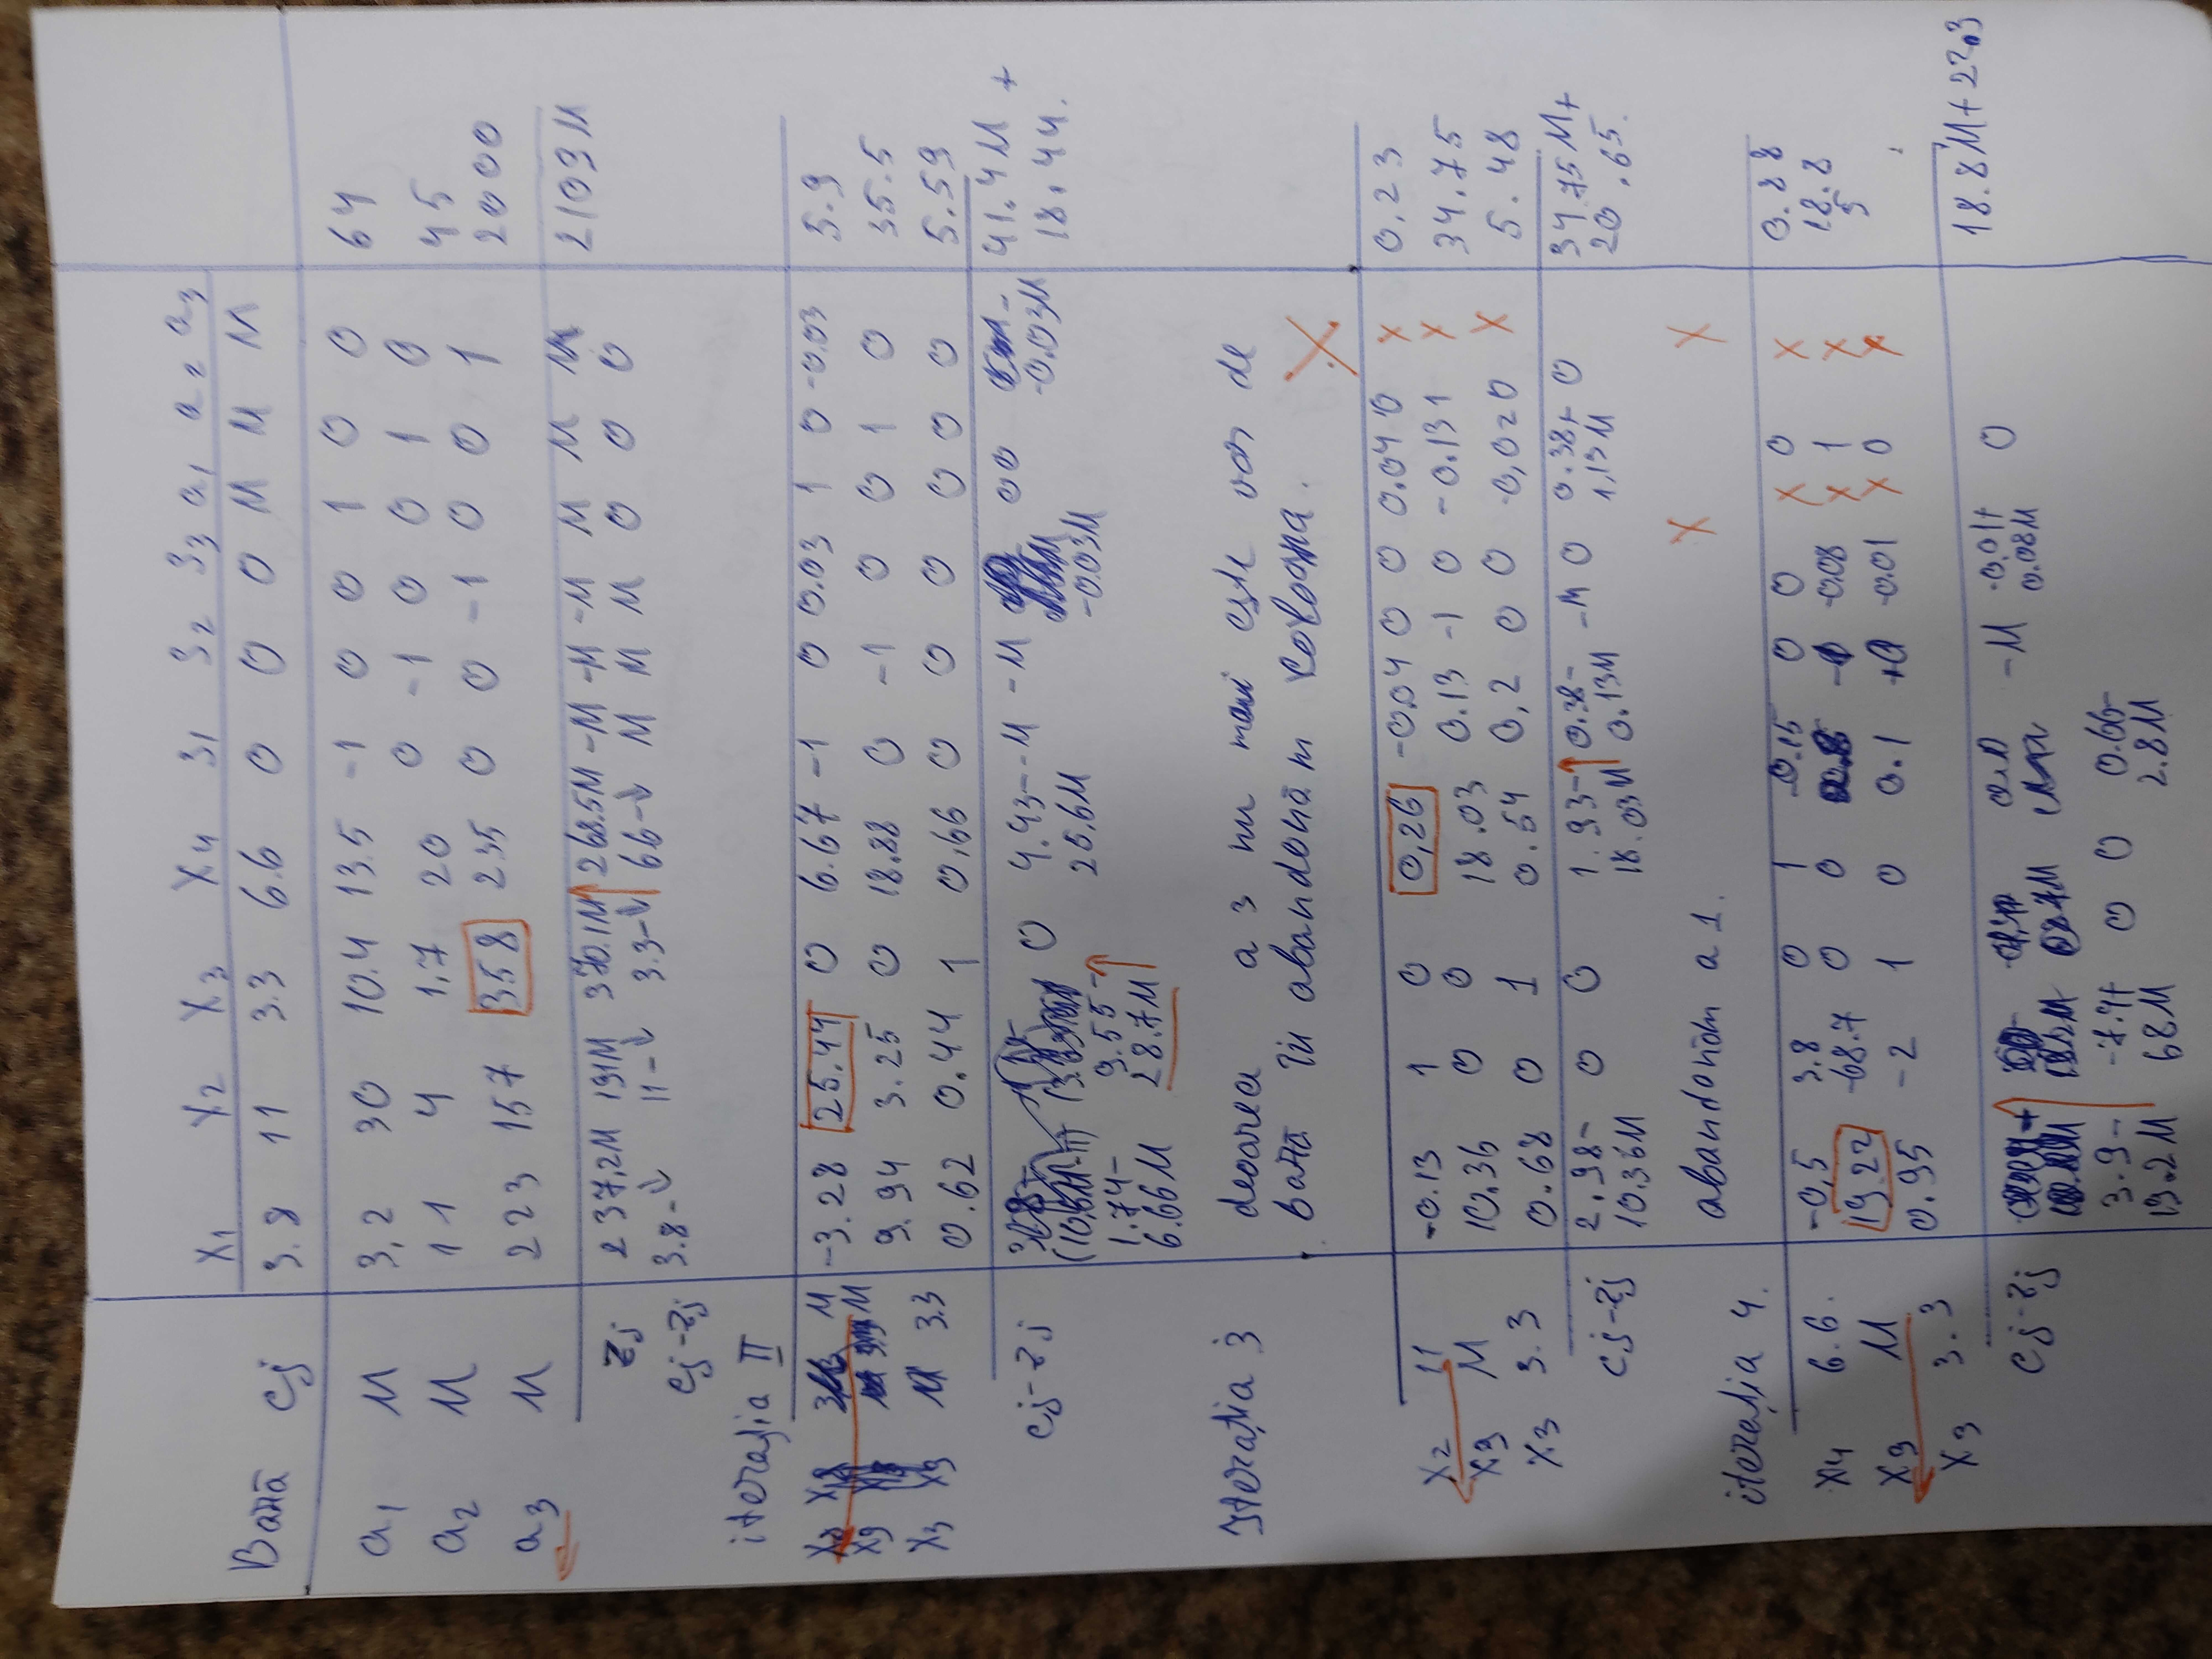
\includegraphics[width=22cm, angle =-90]{4}
\caption{Metoda simplex} 
\label{fig:4}
\end{center}
\end{figure}


\paragraph{}
\begin{figure}[h]
\begin{center}
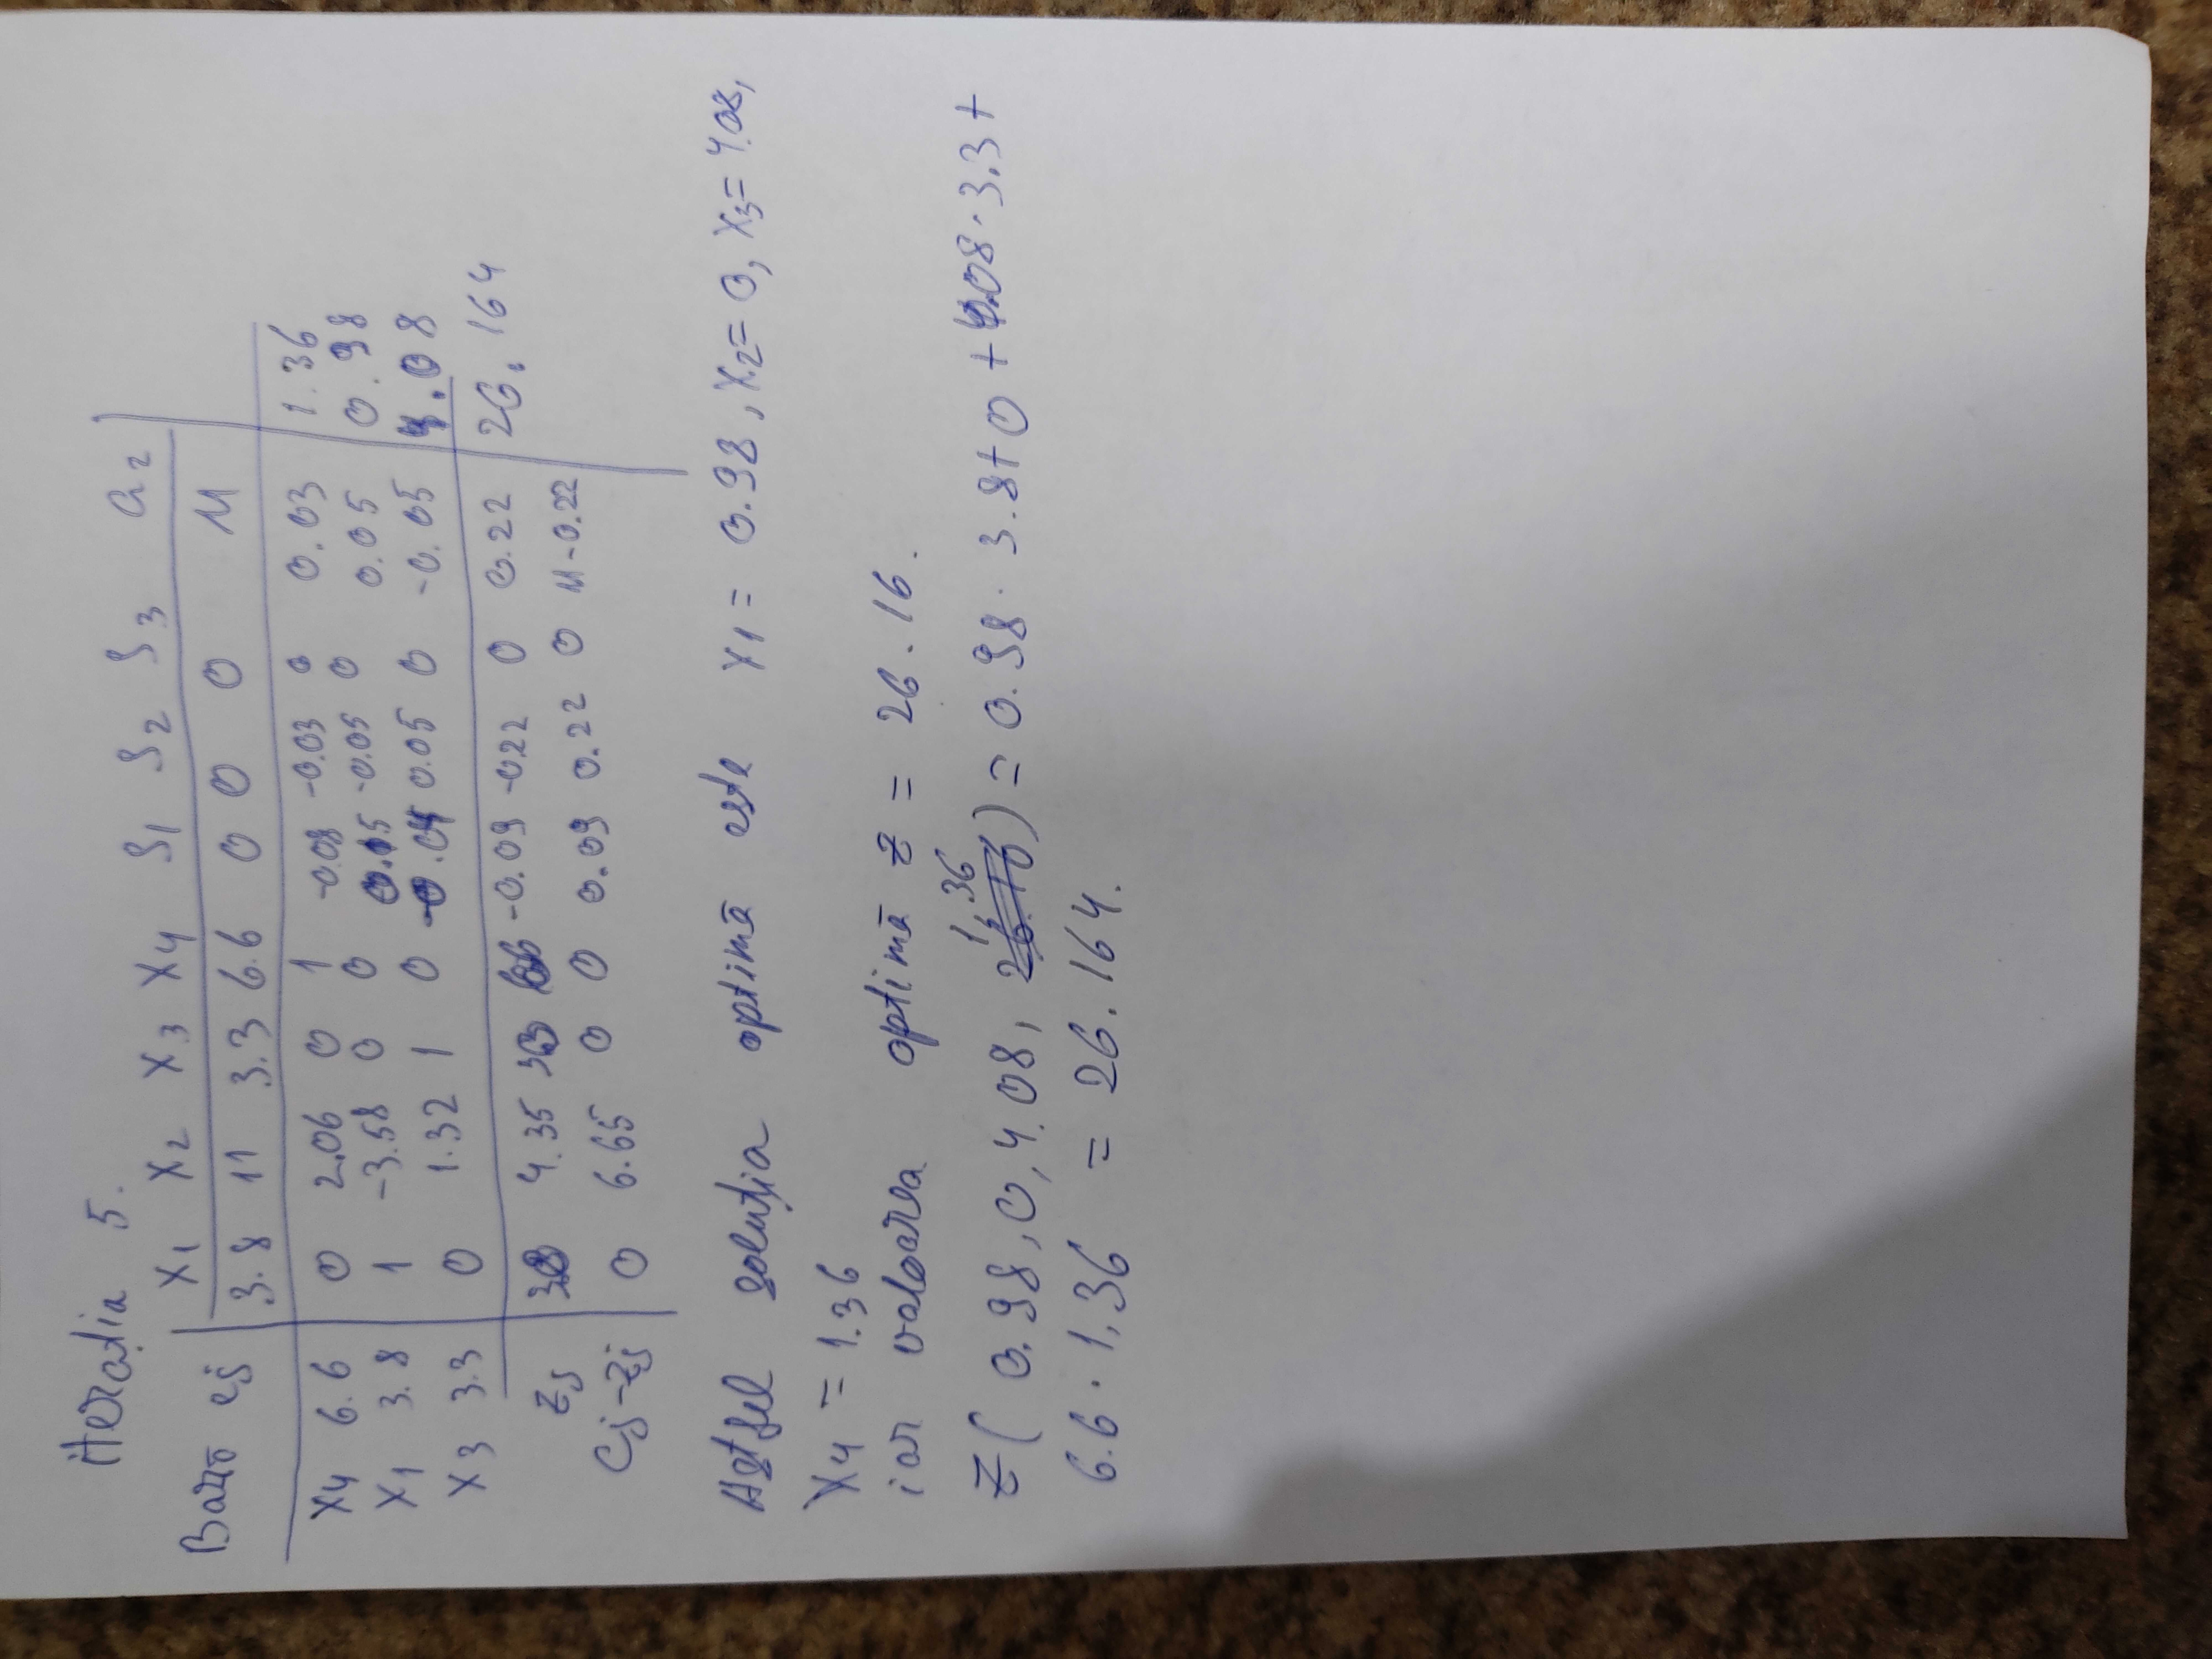
\includegraphics[width=22cm, angle =-90]{5}
\caption{Metoda simplex} 
\label{fig:5}
\end{center}
\end{figure}

